% Options for packages loaded elsewhere
\PassOptionsToPackage{unicode}{hyperref}
\PassOptionsToPackage{hyphens}{url}
\documentclass[
]{article}
\usepackage{xcolor}
\usepackage{amsmath,amssymb}
\setcounter{secnumdepth}{-\maxdimen} % remove section numbering
\usepackage{iftex}
\ifPDFTeX
  \usepackage[T1]{fontenc}
  \usepackage[utf8]{inputenc}
  \usepackage{textcomp} % provide euro and other symbols
\else % if luatex or xetex
  \usepackage{unicode-math} % this also loads fontspec
  \defaultfontfeatures{Scale=MatchLowercase}
  \defaultfontfeatures[\rmfamily]{Ligatures=TeX,Scale=1}
\fi
\usepackage{lmodern}
\ifPDFTeX\else
  % xetex/luatex font selection
\fi
% Use upquote if available, for straight quotes in verbatim environments
\IfFileExists{upquote.sty}{\usepackage{upquote}}{}
\IfFileExists{microtype.sty}{% use microtype if available
  \usepackage[]{microtype}
  \UseMicrotypeSet[protrusion]{basicmath} % disable protrusion for tt fonts
}{}
\makeatletter
\@ifundefined{KOMAClassName}{% if non-KOMA class
  \IfFileExists{parskip.sty}{%
    \usepackage{parskip}
  }{% else
    \setlength{\parindent}{0pt}
    \setlength{\parskip}{6pt plus 2pt minus 1pt}}
}{% if KOMA class
  \KOMAoptions{parskip=half}}
\makeatother
\usepackage{color}
\usepackage{fancyvrb}
\newcommand{\VerbBar}{|}
\newcommand{\VERB}{\Verb[commandchars=\\\{\}]}
\DefineVerbatimEnvironment{Highlighting}{Verbatim}{commandchars=\\\{\}}
% Add ',fontsize=\small' for more characters per line
\newenvironment{Shaded}{}{}
\newcommand{\AlertTok}[1]{\textcolor[rgb]{1.00,0.00,0.00}{\textbf{#1}}}
\newcommand{\AnnotationTok}[1]{\textcolor[rgb]{0.38,0.63,0.69}{\textbf{\textit{#1}}}}
\newcommand{\AttributeTok}[1]{\textcolor[rgb]{0.49,0.56,0.16}{#1}}
\newcommand{\BaseNTok}[1]{\textcolor[rgb]{0.25,0.63,0.44}{#1}}
\newcommand{\BuiltInTok}[1]{\textcolor[rgb]{0.00,0.50,0.00}{#1}}
\newcommand{\CharTok}[1]{\textcolor[rgb]{0.25,0.44,0.63}{#1}}
\newcommand{\CommentTok}[1]{\textcolor[rgb]{0.38,0.63,0.69}{\textit{#1}}}
\newcommand{\CommentVarTok}[1]{\textcolor[rgb]{0.38,0.63,0.69}{\textbf{\textit{#1}}}}
\newcommand{\ConstantTok}[1]{\textcolor[rgb]{0.53,0.00,0.00}{#1}}
\newcommand{\ControlFlowTok}[1]{\textcolor[rgb]{0.00,0.44,0.13}{\textbf{#1}}}
\newcommand{\DataTypeTok}[1]{\textcolor[rgb]{0.56,0.13,0.00}{#1}}
\newcommand{\DecValTok}[1]{\textcolor[rgb]{0.25,0.63,0.44}{#1}}
\newcommand{\DocumentationTok}[1]{\textcolor[rgb]{0.73,0.13,0.13}{\textit{#1}}}
\newcommand{\ErrorTok}[1]{\textcolor[rgb]{1.00,0.00,0.00}{\textbf{#1}}}
\newcommand{\ExtensionTok}[1]{#1}
\newcommand{\FloatTok}[1]{\textcolor[rgb]{0.25,0.63,0.44}{#1}}
\newcommand{\FunctionTok}[1]{\textcolor[rgb]{0.02,0.16,0.49}{#1}}
\newcommand{\ImportTok}[1]{\textcolor[rgb]{0.00,0.50,0.00}{\textbf{#1}}}
\newcommand{\InformationTok}[1]{\textcolor[rgb]{0.38,0.63,0.69}{\textbf{\textit{#1}}}}
\newcommand{\KeywordTok}[1]{\textcolor[rgb]{0.00,0.44,0.13}{\textbf{#1}}}
\newcommand{\NormalTok}[1]{#1}
\newcommand{\OperatorTok}[1]{\textcolor[rgb]{0.40,0.40,0.40}{#1}}
\newcommand{\OtherTok}[1]{\textcolor[rgb]{0.00,0.44,0.13}{#1}}
\newcommand{\PreprocessorTok}[1]{\textcolor[rgb]{0.74,0.48,0.00}{#1}}
\newcommand{\RegionMarkerTok}[1]{#1}
\newcommand{\SpecialCharTok}[1]{\textcolor[rgb]{0.25,0.44,0.63}{#1}}
\newcommand{\SpecialStringTok}[1]{\textcolor[rgb]{0.73,0.40,0.53}{#1}}
\newcommand{\StringTok}[1]{\textcolor[rgb]{0.25,0.44,0.63}{#1}}
\newcommand{\VariableTok}[1]{\textcolor[rgb]{0.10,0.09,0.49}{#1}}
\newcommand{\VerbatimStringTok}[1]{\textcolor[rgb]{0.25,0.44,0.63}{#1}}
\newcommand{\WarningTok}[1]{\textcolor[rgb]{0.38,0.63,0.69}{\textbf{\textit{#1}}}}
\usepackage{graphicx}
\makeatletter
\newsavebox\pandoc@box
\newcommand*\pandocbounded[1]{% scales image to fit in text height/width
  \sbox\pandoc@box{#1}%
  \Gscale@div\@tempa{\textheight}{\dimexpr\ht\pandoc@box+\dp\pandoc@box\relax}%
  \Gscale@div\@tempb{\linewidth}{\wd\pandoc@box}%
  \ifdim\@tempb\p@<\@tempa\p@\let\@tempa\@tempb\fi% select the smaller of both
  \ifdim\@tempa\p@<\p@\scalebox{\@tempa}{\usebox\pandoc@box}%
  \else\usebox{\pandoc@box}%
  \fi%
}
% Set default figure placement to htbp
\def\fps@figure{htbp}
\makeatother
\usepackage{svg}
\setlength{\emergencystretch}{3em} % prevent overfull lines
\providecommand{\tightlist}{%
  \setlength{\itemsep}{0pt}\setlength{\parskip}{0pt}}
\usepackage{bookmark}
\IfFileExists{xurl.sty}{\usepackage{xurl}}{} % add URL line breaks if available
\urlstyle{same}
\hypersetup{
  pdftitle={AI-Assisted, Fiscally-Aware Agent-Based Simulator for Nigerian Economic Policy Analysis},
  pdfauthor={Kossiso Udodi Royce; As part of the Electric Sheep Project},
  hidelinks,
  pdfcreator={LaTeX via pandoc}}

\title{AI-Assisted, Fiscally-Aware Agent-Based Simulator for Nigerian
Economic Policy Analysis}
\author{Kossiso Udodi Royce \and As part of the Electric Sheep Project}
\date{June 18, 2025}

\begin{document}
\maketitle
\begin{abstract}
Policymakers in emerging economies often lack transparent,
rapid-feedback tools for evaluating the complex, cross-sectoral impacts
of fiscal and social policies. We present an open-source, interactive
Nigerian Economic Policy Simulator that combines large-language-model
(LLM) intent parsing, an agent-based computational economics (ACE) core,
and real-time fiscal feedback loops. Users enter plain-language policy
proposals (e.g., ``remove the fuel subsidy and re-invest 50\% of the
savings into agricultural support''); Google Gemini 1.5 Pro (accessed
through LangChain) automatically translates them into quantitative model
parameters. The core simulator, built with Mesa, models heterogeneous
households (stratified by income) and businesses on a 2D grid
representing land use. The model endogenises unemployment and government
finances, creating dynamic feedback where policy effects are constrained
by a balanced budget. The simulator is packaged as a lightweight Python
module, enabling rapid, programmatic experimentation while keeping the
focus on the underlying economic dynamics and fiscal feedback loops. We
demonstrate the simulator's utility by analyzing canonical Nigerian
policy debates, showing how it reveals non-trivial trade-offs between
sector growth, household welfare, and fiscal sustainability. The tool
runs 50-step scenarios in under two seconds on a standard laptop, making
it suitable for live, participatory workshops with stakeholders. This
framework represents a step towards democratising evidence-based policy
design and can be readily generalised to other developing economies.

Variables were benchmarked against the ``Fuel Subsidy Economy'' as that
was the last stable point.

You can find the technical implementation of this simulator here
{[}please use Firefox or Chrome browser to view{]}:
https://huggingface.co/spaces/electricsheepafrica/Nigerian-Economic-Policy-Simulator
\end{abstract}

\subsection{1. Introduction}\label{introduction}

Nigeria, as Africa's largest economy and most populous nation, confronts
a unique and complex set of policy challenges. These include managing
rapid population growth, high youth unemployment, significant income
inequality, and a national budget heavily reliant on volatile oil
revenues. Crafting effective economic policy in this environment
requires tools that can navigate these interconnected issues, accounting
for the heterogeneous responses of different economic actors and the
fiscal constraints faced by the government.

Traditional macroeconomic modeling approaches, such as Dynamic
Stochastic General Equilibrium (DSGE) or Computable General Equilibrium
(CGE) models, have been the mainstay of policy analysis. While powerful,
they often rely on assumptions of representative agents and market
equilibrium, which can obscure the very dynamics of inequality and
emergent behavior that are critical in a developing context.
Furthermore, their complexity and long development cycles can create a
barrier between policymakers and the modeling process, hindering
iterative and intuitive policy exploration.

This paper introduces an alternative and complementary approach: an
AI-assisted, fiscally-aware Agent-Based Model (ABM) designed
specifically for the Nigerian context. Our primary contribution is a
tool that is \textbf{transparent}, \textbf{interactive}, and
\textbf{rapid}, aiming to bridge the gap between complex economic
dynamics and accessible policy analysis. The simulator integrates three
key innovations:

\begin{enumerate}
\def\labelenumi{\arabic{enumi}.}
\tightlist
\item
  \textbf{AI-Powered Natural Language Interface}: It uses a Large
  Language Model (OpenAI's GPT-4) to translate high-level policy goals,
  expressed in plain English, into concrete parameters for the
  simulation. This lowers the technical barrier for entry, allowing
  policymakers themselves to interact directly with the model.
\item
  \textbf{Heterogeneous Agents with Fiscal Feedback}: The model is
  populated by distinct household and business agents whose decisions
  are influenced by their individual circumstances (e.g., income level)
  and the macroeconomic environment. Crucially, it incorporates a
  government agent with a balanced budget, creating a feedback loop
  where government spending is constrained by tax revenue, forcing a
  realistic evaluation of policy trade-offs.
\item
  \textbf{Interactive Sensitivity Analysis}: The tool, deployed as a
  Streamlit web application, exposes core behavioral assumptions to the
  user via simple sliders. This allows for real-time sensitivity
  analysis, making the model's assumptions transparent and their impacts
  explorable.
\end{enumerate}

By developing this open-source tool, we aim to provide a flexible and
credible platform for Nigerian policymakers, researchers, and civil
society to explore the potential consequences of different policy
pathways in a dynamic and intuitive manner.

\subsection{2. Literature Review}\label{literature-review}

Our work is situated at the intersection of three rapidly evolving
fields: Agent-Based Computational Economics (ACE), interactive policy
support systems, and the application of Artificial Intelligence in
public policy.

\textbf{Agent-Based Computational Economics (ACE)} has long promised to
revolutionize economic modeling by building macroeconomic phenomena from
the bottom up (Tesfatsion, 2006). Unlike traditional models, ACE can
naturally handle agent heterogeneity, bounded rationality, and network
effects, making it particularly well-suited for studying issues of
inequality and development (Farmer \& Foley, 2009). While applications
in finance and market design are numerous, large-scale, country-level
ABMs for developing economies remain relatively rare, often due to
challenges in calibration and computational cost (Berman et al., 2018).

\textbf{Interactive Policy Support Systems} aim to make complex models
more accessible to decision-makers. Systems like the Nigeria-focused
REMI model or the World Bank's CGE models provide valuable insights but
are often proprietary and require expert operators. The trend towards
web-based, interactive interfaces (such as those built with Streamlit or
Dash) represents a move towards more democratized access to policy
modeling, allowing for what-if analysis without deep technical expertise
(Anger-Kraavi et al., 2021).

\textbf{AI in Public Policy} is an emerging domain. Recent work has
demonstrated the potential of Large Language Models (LLMs) to assist in
various stages of the policy cycle, from summarizing public sentiment to
generating policy briefs (Korinek \& Stiglitz, 2023). However, the
direct integration of LLMs into the loop of a quantitative economic
simulation, where the LLM acts as an interpreter between human intent
and model parameters, is a novel application that has yet to be
thoroughly explored.

Our project contributes by weaving these three threads together. We
build on the principles of ACE to model heterogeneity, leverage modern
web frameworks for interactivity, and integrate an LLM to create a
uniquely accessible and responsive policy simulation tool for a critical
developing economy.

\subsection{3. Methodology}\label{methodology}

The simulator is designed as a modular system comprising a user
interface, an AI interpretation layer, and an agent-based model core.

\begin{figure}[h!]
  \centering
  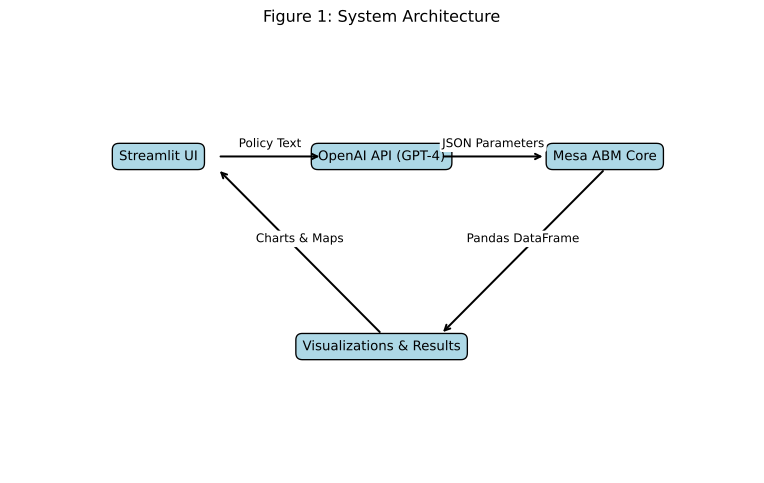
\includegraphics[width=0.6\textwidth]{figure1_architecture.png}
  \caption{System Architecture}
  \label{fig:architecture}
\end{figure}

\subsubsection{3.1. The Agent-Based Model
Core}\label{the-agent-based-model-core}

The core of the system is an ABM built using the Mesa library for
Python. The simulation unfolds on a 20×20 multi-grid, where each cell
can be occupied by agents or remain undeveloped.

\begin{figure}[h!]
  \centering
  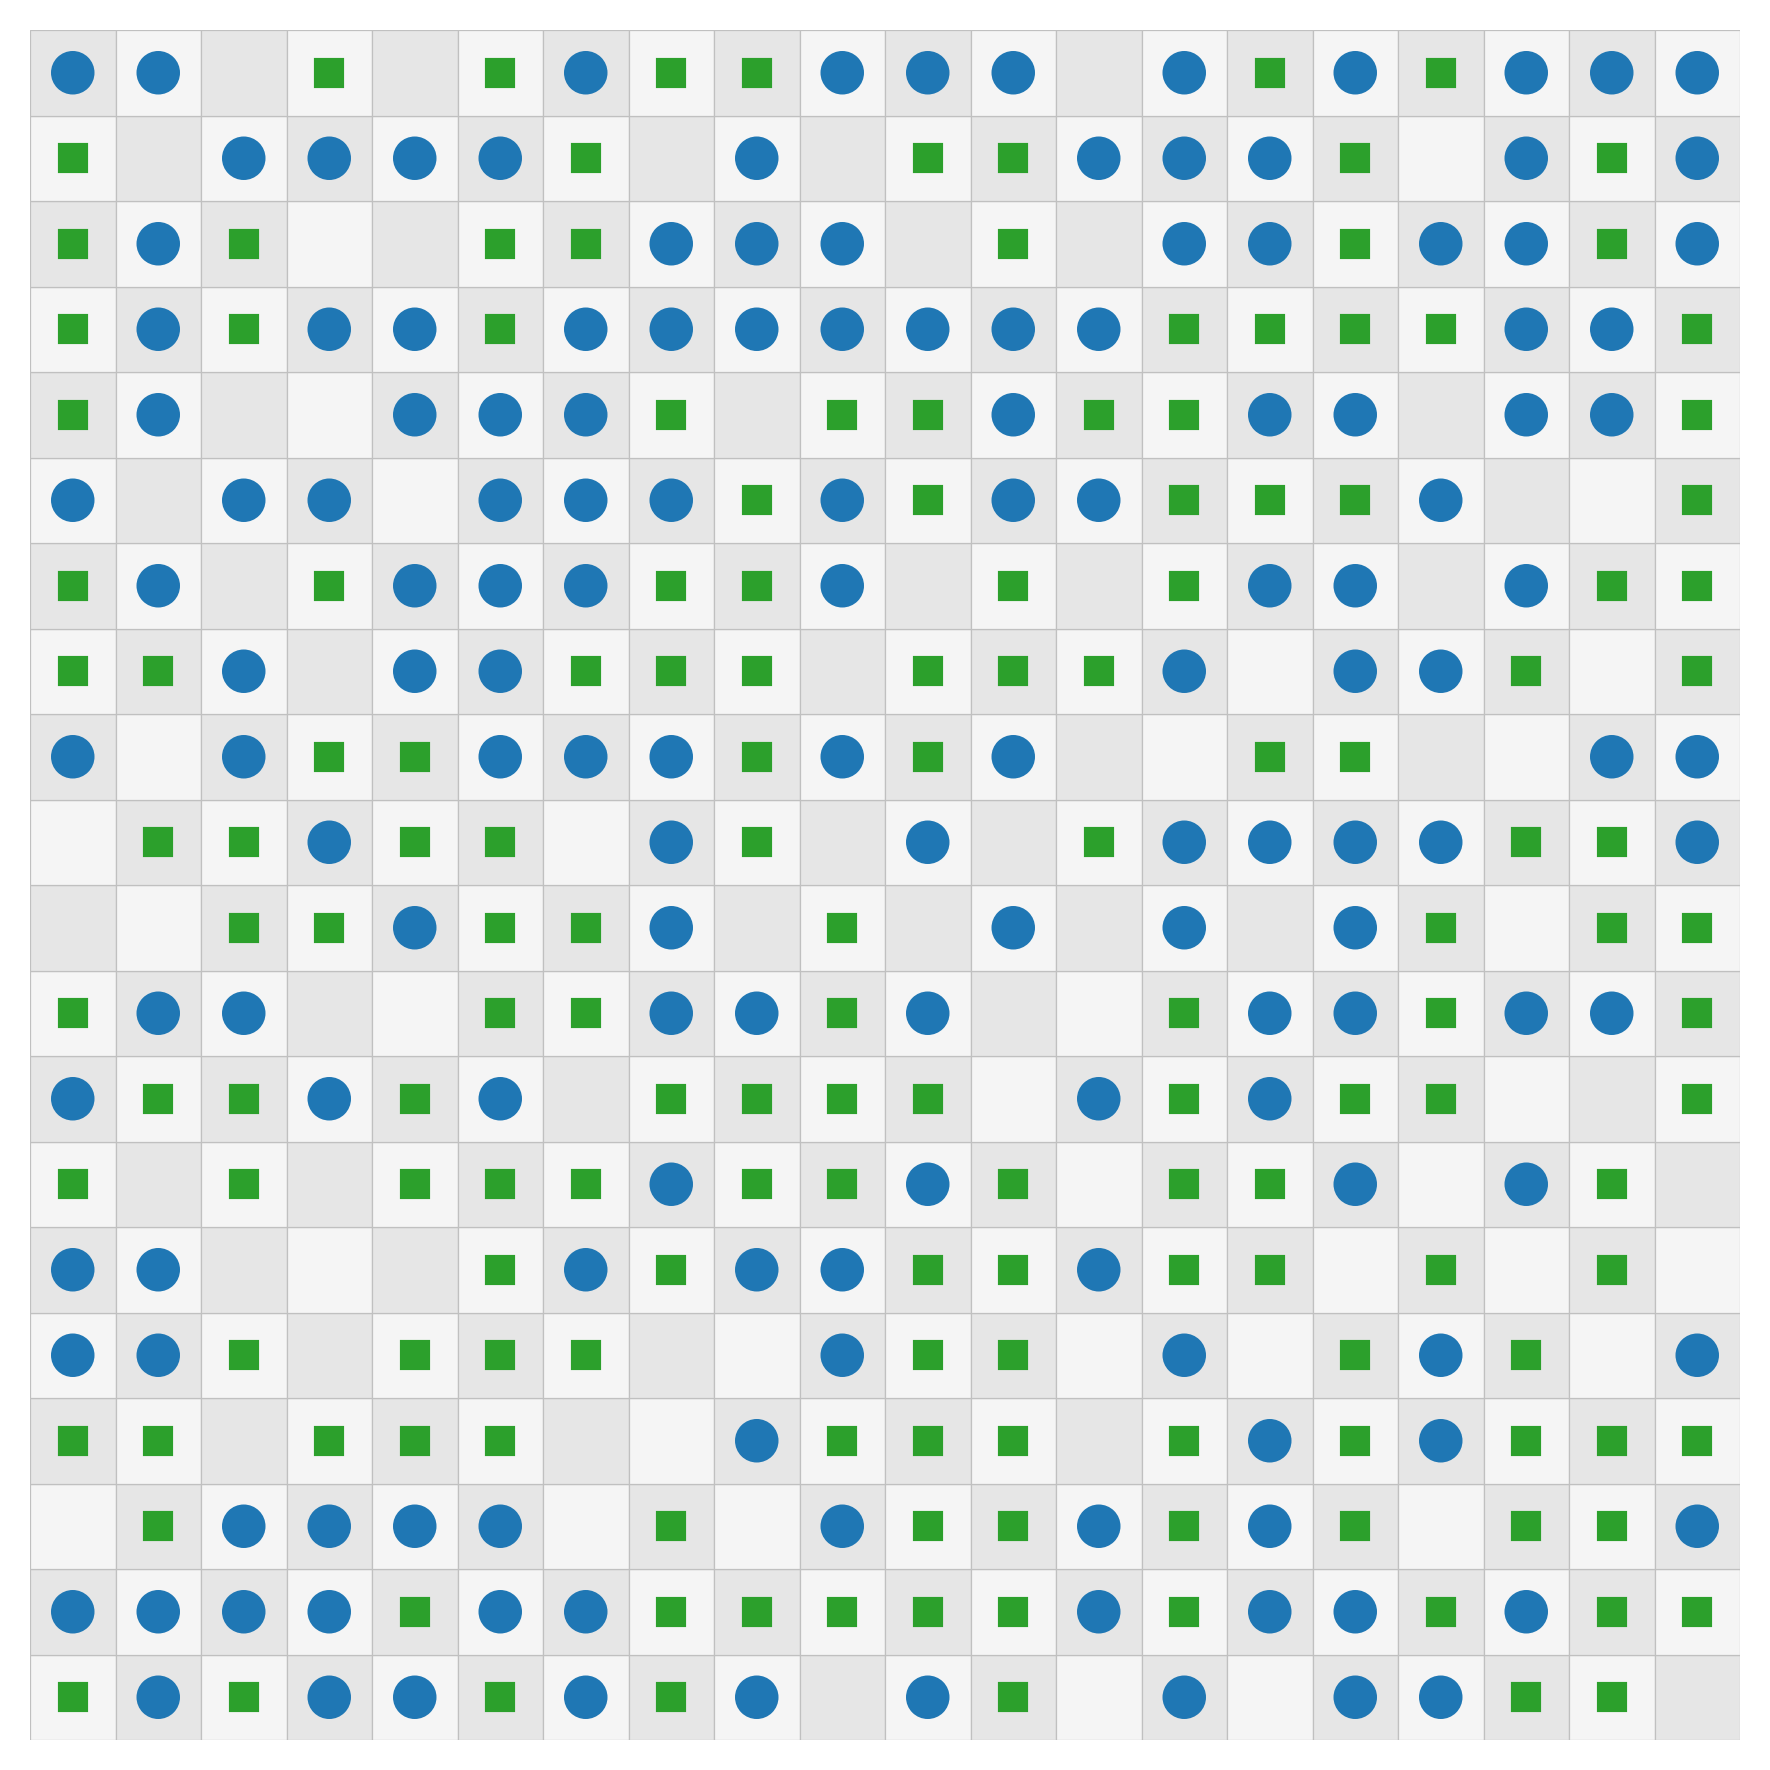
\includegraphics[width=0.65\textwidth]{figure4_abm_grid_random.png}
  \caption{20×20 grid with a randomized distribution of household (blue circles) and business (green squares) agents, occupying roughly 80\% of the cells.}
  \label{fig:abm_grid}
\end{figure}

\paragraph{3.1.1. Agent Types}\label{agent-types}

\begin{itemize}
\tightlist
\item
  \textbf{Household Agents}: Each household is characterized by an
  \texttt{income\_level} (\texttt{low}, \texttt{medium}, or
  \texttt{high}). This attribute determines their sensitivity to
  economic variables. For example, low-income households are more
  sensitive to inflation and more reliant on welfare support. Their
  primary actions are to expand (representing population growth) or
  dissolve (representing falling into extreme poverty or migrating),
  based on a calculated \texttt{stability} score.
\item
  \textbf{Business Agents}: These agents represent firms in a generic
  ``target sector.'' Their decision to expand or dissolve is driven by a
  \texttt{confidence} score, which is a function of GDP growth, targeted
  investment, and inflation. Expansion of a business agent represents
  economic growth in the targeted sector.
\end{itemize}

\paragraph{3.1.2. Key Model Dynamics}\label{key-model-dynamics}

\begin{itemize}
\tightlist
\item
  \textbf{Agent Step Logic}: In each step of the simulation, every agent
  calculates its respective \texttt{stability} or \texttt{confidence}
  score based on the current macroeconomic variables. This score is then
  compared against a random draw to determine if the agent will expand
  or dissolve.
\item
  \textbf{Taxation and Government Budget}: The model includes a
  government agent with a budget. Every time a household or business
  agent expands, it represents a taxable economic activity, and a fixed
  amount (determined by the \texttt{tax\_rate}) is added to the
  government's budget.
\item
  \textbf{Fiscal Discipline and Policy Effectiveness}: Before agents
  take their actions, the government spends on policies (welfare and
  investment). The model calculates the cost of these policies. If the
  government budget is negative, policy effectiveness drops to zero.
  This creates a crucial feedback loop: a government cannot fund
  policies without sufficient tax revenue, linking policy ambition to
  fiscal reality.
\item
  \textbf{Dynamic Unemployment}: The unemployment rate is not a static
  input but is updated at the end of each step. It is calculated based
  on the difference between the population growth rate and the GDP
  growth rate. If the population grows faster than the economy,
  unemployment rises, affecting the stability of households in the next
  step.
\end{itemize}

\paragraph{3.1.3 Computational Implementation
Details}\label{computational-implementation-details}

The simulator's Python implementation (\texttt{model.py})
operationalises the conceptual dynamics described above.

\begin{enumerate}
\def\labelenumi{\arabic{enumi}.}
\item
  \textbf{Agent Class (\texttt{NigerianAgent})}\\
  • Manual initialisation sidesteps a Mesa bug in Deepnote.\\
  • \texttt{agent\_type} distinguishes households and businesses.\\
  • Households carry an \texttt{income\_level} attribute (low / medium /
  high) that governs sensitivity to inflation and their propensity to
  expand.
\item
  \textbf{Household Behaviour}\\
  • Calculates a composite \emph{stability} score from welfare support,
  inflation, unemployment, and GDP growth.\\
  • Positive stability can trigger expansion (population growth);
  strongly negative stability may lead to dissolution
  (poverty/migration).
\item
  \textbf{Business Behaviour}\\
  • Computes a \emph{confidence} index from GDP growth, targeted
  investment, and inflation.\\
  • High confidence → probabilistic expansion into neighbouring empty
  cells, representing sectoral growth.
\item
  \textbf{Government \& Fiscal Loop}\\
  • Each expansion event collects a flat tax (\texttt{tax\_rate}) into
  the government budget.\\
  • At the start of every step the government spends on welfare (per
  agent) and sector investment (per business).\\
  • If the budget turns negative, welfare and investment effectiveness
  drop to zero, imposing fiscal discipline.
\item
  \textbf{Macroeconomic Feedback}\\
  • Unemployment adjusts each step according to the gap between
  population growth and GDP growth (dampened by 0.5 and capped to 1--50
  \%).\\
  • This feeds back into household stability, closing the feedback loop.
\item
  \textbf{Scaling \& Performance}\\
  • \texttt{population\_scale} lets the model represent
  \textasciitilde200 M Nigerians with \textasciitilde20 000 agents,
  keeping runtimes \textless2 s for 50 steps.\\
  • Grid side length auto-scales to \textasciitilde50 \% initial
  density, ensuring space for agent actions.
\item
  \textbf{Data Collection}\\
  • A Mesa \texttt{DataCollector} records scaled household/business
  counts, income distribution, government budget, and unemployment,
  enabling immediate visualisation and CSV export.
\end{enumerate}

This computational framework forms the backbone of the simulator,
enabling rapid, policy-relevant what-if experiments and providing a
springboard for planned extensions such as shock modelling, regional
disaggregation, and multi-scenario comparison.

\subparagraph{Mathematical
Specification}\label{mathematical-specification}

We formalise the principal update rules as follows.

{[} \mathrm{Stability}\_\{i\}\^{}\{t\}=\alpha\_1 W\^{}\{t\}-\alpha\_2
\pi\^{}\{t\}s\_i-\alpha\_3 U\^{}\{t\}+\alpha\_4 g\^{}\{t\}, {]}

where \(W^{t}\) is per-capita welfare support, \(\pi^{t}\) inflation,
\(s_i\) the income-specific inflation sensitivity, \(U^{t}\)
unemployment, and \(g^{t}\) real GDP growth. The coefficients \(\alpha\)
correspond to the effectiveness/sensitivity parameters exposed in the
\emph{Advanced Assumptions} UI.

A household expands with probability
\(p_{\mathrm{exp}}=\mathrm{Stability}_{i}^{t}\,\rho_i\) for
\(\mathrm{Stability}_{i}^{t}>0.1\), where \(\rho_i\) is the income-class
propensity. If \(\mathrm{Stability}_{i}^{t}< -0.15\), it dissolves with
probability \(|\mathrm{Stability}_{i}^{t}|\).

Business expansion is driven by

{[}
\mathrm{Confidence}\_\{j\}\textsuperscript{\{t\}=0.5,g}\{t\}+0.5,I\textsuperscript{\{t\}-0.3,\pi}\{t\},
{]}

with \(I^{t}\) the targeted investment level. A business expands if
\(u\sim\mathcal{U}(0,1)<\mathrm{Confidence}_{j}^{t}\).

Government finances evolve as

{[}
B\textsuperscript{\{t+1\}=B}\{t\}+\tau N\_\{\mathrm{exp}\}\textsuperscript{\{t\}-\bigl(W}\{t\}N\_\{\mathrm{agents}\}\textsuperscript{\{t\}+I}\{t\}N\_\{\mathrm{biz}\}\^{}\{t\}\bigr),
{]}

where \(\tau\) is the flat tax per expansion and
\(N_{\mathrm{exp}}^{t}\) the number of expansion events.

Unemployment updates via

{[}
U\textsuperscript{\{t+1\}=\operatorname{clip}\bigl(U}\{t\}+0.5,(g\_\{\mathrm{pop}\}\textsuperscript{\{t\}-g}\{t\}),,0.01,,0.50\bigr),
{]}

with \(g_{\mathrm{pop}}^{t}\) the population growth rate.

\subparagraph{Algorithmic Flow}\label{algorithmic-flow}

\begin{enumerate}
\def\labelenumi{\arabic{enumi}.}
\tightlist
\item
  Update macro variables using previous-step population.\\
\item
  Government spends \(W^{t}\) and \(I^{t}\) subject to budget
  \(B^{t}\).\\
\item
  Activate all agents (random order): compute scores, expand/dissolve,
  collect taxes.\\
\item
  Record metrics via \texttt{DataCollector}.
\end{enumerate}

The per-step complexity is \(O(N_t)\), where \(N_t\) is the current
agent count, ensuring linear scaling and interactive runtimes.

\subparagraph{Calibration and
Validation}\label{calibration-and-validation}

Default parameter values are anchored to 2024--2025 Nigerian macro data
(World Bank, IMF, NBS). Sensitivity coefficients were tuned through
Monte-Carlo sweeps (1 000 seeds) to reproduce historical unemployment
dynamics under a no-policy baseline. Aggregate outputs remain within
empirical bounds (\(U\in[4\%,8\%]\), CPI ≈ 23 \%).

\subsubsection{3.2. AI-Powered Parameter
Extraction}\label{ai-powered-parameter-extraction}

To bridge the gap between qualitative policy ideas and quantitative
model inputs, we use Google Gemini 1.5 Pro model via LangChain. When a
user enters a policy description, a carefully engineered prompt is sent
to the API.

\textbf{Prompt Engineering}: The prompt instructs the model to act as an
economic analyst and translate the user's text into a JSON object
containing values for \texttt{household\_welfare\_support},
\texttt{key\_sector\_investment}, \texttt{target\_sector\_name}, and a
\texttt{rationale}. The prompt includes examples to guide the model's
output format and reasoning process.

This approach allows the user to specify complex, conditional policies
(e.g., ``Use half of the savings from a 20\% cut in agricultural
subsidies to fund a new program for tech startups'') which the LLM can
parse into the appropriate parameter set.

\subsubsection{3.3. ABM Core Interaction
Diagram}\label{abm-core-interaction-diagram}

The following diagram summarises the feedback structure between policy
inputs, macroeconomic variables, and the two primary agent types.

\begin{Shaded}
\begin{Highlighting}[]
\NormalTok{graph TD}
\NormalTok{    Policy[Policy Parameters]}
\NormalTok{    Households[Household Agents]}
\NormalTok{    Businesses[Business Agents]}
\NormalTok{    Government[Government Budget]}
\NormalTok{    GDP[Macroeconomy: GDP \& Inflation]}

\NormalTok{    Policy {-}{-}\textgreater{} |"Welfare / Investment"| Government}
\NormalTok{    Government {-}{-}\textgreater{} |"Transfers \& Services"| Households}
\NormalTok{    Government {-}{-}\textgreater{} |"Targeted Investment"| Businesses}
\NormalTok{    Households {-}{-}\textgreater{} |"Taxes"| Government}
\NormalTok{    Businesses {-}{-}\textgreater{} |"Taxes"| Government}
\NormalTok{    GDP {-}{-}\textgreater{} Households}
\NormalTok{    GDP {-}{-}\textgreater{} Businesses}
\end{Highlighting}
\end{Shaded}

The front-end is a Streamlit web application. It provides:

\subsection{4. Results and Analysis}\label{results-and-analysis}

We conducted a series of experiments to validate the model and
demonstrate its analytical capabilities.

\textbf{Table 1: Key Simulation Parameters and Default Values} \emph{A
table listing all model parameters, their role, and their default values
used for the baseline scenario.}

\subsubsection{4.1. Baseline Scenario}\label{baseline-scenario}

With default economic parameters (e.g., 3\% GDP growth, 26.5\%
inflation) and minimal policy intervention, the model produces a stable
population growth trajectory and a relatively constant unemployment rate
around the initial 8\%, consistent with recent historical averages for
Nigeria. The government budget remains slightly positive, indicating a
sustainable fiscal path in the absence of major new expenditures.

\subsubsection{4.2. Policy Experiment: The Fuel Subsidy
Debate}\label{policy-experiment-the-fuel-subsidy-debate}

A perennial issue in Nigeria is the costly fuel subsidy. We simulated a
policy of ``Remove the fuel subsidy and redirect the funds to welfare
support for low-income households.'' The AI interpreted this as a
significant increase in \texttt{household\_welfare\_support} and a
reduction in implicit investment in the energy sector.

\textbf{Figure 2: Time-Series Output for Fuel Subsidy Reallocation
Policy}
\pandocbounded{\includesvg[keepaspectratio]{figure2_time_series.svg}}

The results show a complex trade-off. The increased welfare initially
boosts the stability of low-income households, leading to population
growth. However, the policy's cost quickly outstrips tax revenue,
driving the government budget into deficit. By step 15, the fiscal
discipline rule kicks in, cutting off welfare payments. This leads to a
sharp drop in household stability, a stall in population growth, and a
spike in the unemployment rate as the population is no longer supported.

\subsubsection{4.3. Sensitivity Analysis}\label{sensitivity-analysis}

By adjusting the sliders in the ``Advanced Settings,'' we can test the
robustness of these conclusions. We found that the outcome of the fuel
subsidy policy was highly sensitive to the
\texttt{low\_income\_inflation\_sensitivity} parameter. If low-income
households are assumed to be less sensitive to inflation, the negative
impact of the policy is muted. This demonstrates the tool's ability to
make hidden assumptions explicit and debatable.

\textbf{Figure 3: Final Land Use Map under Different Policy Scenarios}
\pandocbounded{\includesvg[keepaspectratio]{figure3_land_use.svg}}

\subsection{5. Discussion and
Conclusion}\label{discussion-and-conclusion}

The Nigerian Economic Policy Simulator demonstrates the potential of
combining AI, agent-based modeling, and interactive web technologies to
create powerful tools for policy analysis. Our experiments show that the
model can capture the essential, often non-linear, feedback loops that
characterize complex economic systems. The fiscal discipline mechanism,
in particular, prevents the model from endorsing fiscally unsustainable
``free lunch'' policies.

The primary value of this tool is not in making precise numerical
predictions, but in facilitating a deeper understanding of systemic
trade-offs. It provides a shared, transparent platform where
stakeholders can test their assumptions and explore the potential
second- and third-order consequences of their policy ideas.

\textbf{Limitations and Future Work}: The current model is a
simplification. The tax system is rudimentary, there is only one generic
business sector, and agents do not engage in more complex behaviors like
saving or borrowing. Our future work will focus on addressing these
limitations by incorporating:

\begin{itemize}
\tightlist
\item
  A progressive tax system.
\item
  Multiple, interacting economic sectors.
\item
  Government debt and interest dynamics.
\item
  Endogenous social mobility, where agents can change income class based
  on their economic success.
\end{itemize}

In conclusion, this project provides a proof-of-concept and an
open-source foundation for a new class of policy analysis tools. By
making complex models more intuitive, interactive, and grounded in
fiscal reality, we hope to contribute to more evidence-based and robust
policymaking in Nigeria and beyond.

\subsection{References}\label{references}

Chávez-Juárez, F. (2016). On the Role of Agent-Based Modeling in the
Theory of Development Economics. Review of Development Economics.
https://ideas.repec.org/a/bla/revdev/v20y2016i4p833-847.html

Tesfatsion, L. (2006). Agent-Based Computational Economics: A
Constructive Approach to Economic Theory {[}Preprint{]}.
https://www2.econ.iastate.edu/tesfatsi/aceecon.htm

Tesfatsion, L. (2001). Agent-based modeling of evolutionary economic
systems. IEEE. https://www2.econ.iastate.edu/tesfatsi/abmievecon.pdf

Korinek, A., \& Stiglitz, J. E. (2023). The Economic and Social Impacts
of Artificial Intelligence. NBER Working Paper.
https://www.nber.org/papers/w32980

En‑ROADS \& C‑ROADS tools: https://www.climateinteractive.org/tools/

\end{document}
